\subsection{Vergleich mehrerer Algorithmen}
\label{framework:bechmark:sacabench-batch}

\begin{wrapfigure}{R}{.5\textwidth}
	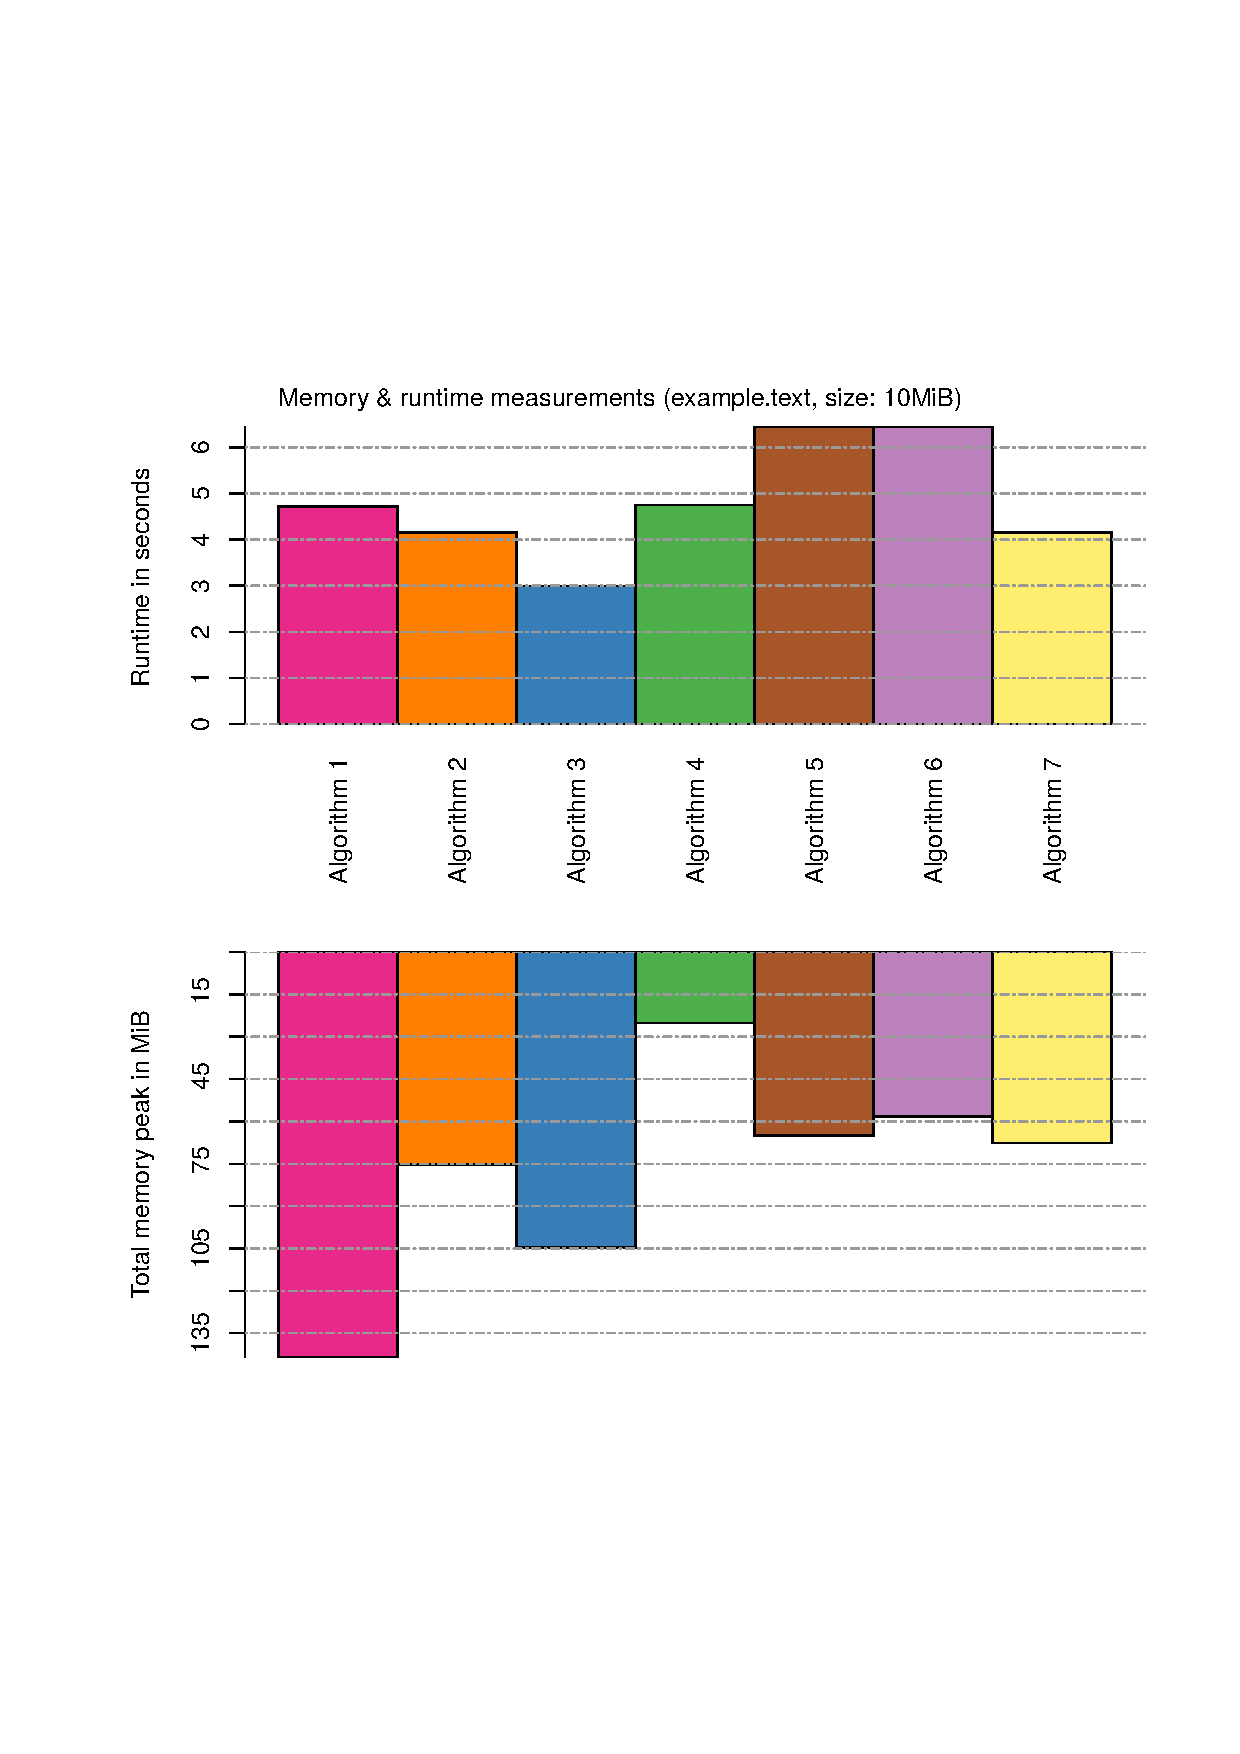
\includegraphics[page = 1, width=.5\textwidth]{kapitel/3_framework/benchmark/sacabench-batch/beispiel_batch_saeule.pdf}
	\caption{Messergebnisse mehrerer Algorithmen}
	\label{pdf:benchmark:batch:saeule}
\end{wrapfigure}

Ist jedoch nach den Messergebnissen aller vorhandenen Algorithmen in dem \sacabench-Framework gefragt, wird der Befehl \texttt{sacabench batch} mit der Option \termfont{-z} oder \termfont{-{}-rplot} verwendet. Dabei wird von jedem Algorithmus die Laufzeit und der Spei\-cher\-ver\-brauch gemessen. Diese Messungen schaffen einen Überblick aller Algorithmen. Anders als bei den Ergebnissen einzelner Algorithmen, wird hierbei der Übersicht halber auf die Unterteilung in Phasen verzichtet. Die dabei erstellte \texttt{PDF}-Datei enthält sieben Seiten.

Die \cref{pdf:benchmark:batch:saeule} zeigt die erste Seite der \texttt{PDF}-Datei. Auf dieser sind zwei Säulendiagramme abgebildet. Das obere Diagramm repräsentiert die jeweiligen Laufzeiten und das untere Diagramm zeigt den maximalen Spei\-cher\-ver\-brauch inklusive des Ausgangstextes -- beides jeweils in passenden Einheiten. Jede einzelne Säule eines Diagramms steht für einen Algorithmus. In der Mitte beider Diagramme sind die dazugehörigen Namen der Algorithmen wiederzufinden. Auf der ersten Seite sind diese Algorithmen aufsteigend nach Namen sortiert. Diese Reihenfolge ermöglicht einen besseren Vergleich der Messergebnisse unserer Implementierungen mit den Ergebnissen der Referenzimplementierungen, da diese bis auf das Suffix \texttt{\_ref} den gleichen Namen haben und somit nebeneinander aufgelistet werden.

Auf der zweiten Seite sind die selben Messungen wiederzufinden, jedoch ist das Säulendiagramm aufsteigend nach der Laufzeit umsortiert worden. Dadurch lassen sich die Laufzeiten der Algorithmen besser miteinander vergleichen.

Auf der dritten Seite ist die Sortierung der Säulen aufsteigend nach dem maximalen Spei\-cher\-ver\-brauch gewählt worden. Durch diese Reihenfolge lassen sich bessere Vergleiche für ähnliche Werte des Spei\-cher\-ver\-brauchs ziehen.

\begin{wrapfigure}{R}{.5\textwidth}
	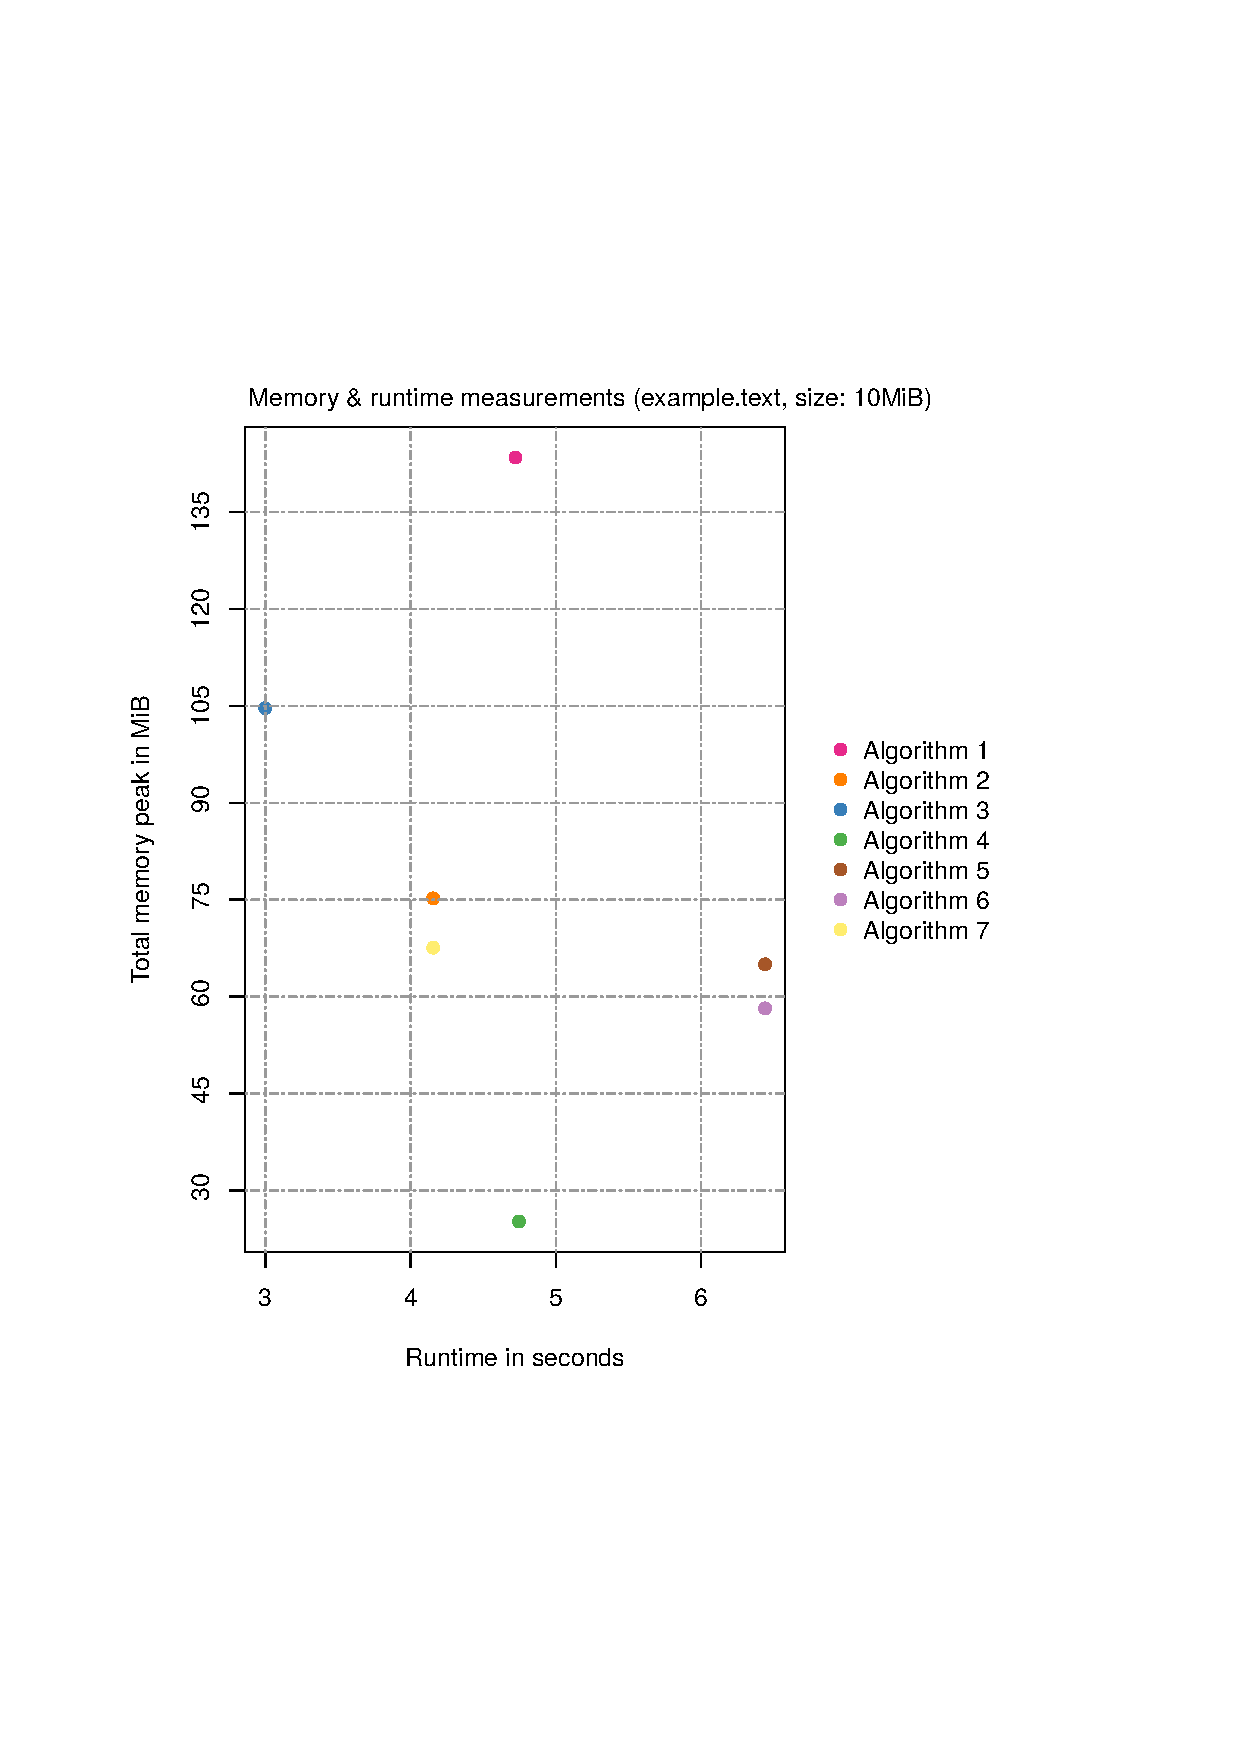
\includegraphics[page = 1, width=.5\textwidth]{kapitel/3_framework/benchmark/sacabench-batch/beispiel_batch_streu.pdf}
	\caption{Messergebnisse mehrerer Algorithmen}
	\label{pdf:benchmark:batch:streu}
\end{wrapfigure}

Die \cref{pdf:benchmark:batch:streu} zeigt die vierte Seite der \texttt{PDF}-Datei. Auf dieser ist statt eines Säulendiagramms ein Streudiagramm zum Einsatz gekommen. Hierbei handelt  es sich lediglich um eine andere Darstellungsform. Auf der X-Achse befindet sich die Skala für die Laufzeit und auf der Y-Achse die Skala für den maximalen Spei\-cher\-ver\-brauch von jedem Algorithmus für einen gegebenen Text. Rechts neben dem Diagramm ist die dazugehörige Legende wiederzufinden.

Auf der fünften Seite ist erneut ein Streudiagramm zu sehen. Jedoch ist dieses Mal lediglich die Pareto-Front eingezeichnet. In unserem Fall bedeutet das, dass ein zwei-dimensionaler Punkt dem Messergebnis eines Algorithmus entspricht, wobei eine Dimension der Laufzeit und die andere Dimension dem maximalen Spei\-cher\-ver\-brauch entspricht. Ein Algorithmus gehört somit zu der Pareto-Front, wenn kein anderer Algorithmus sowohl eine kürzere Laufzeit als auch einen kleineren maximalen Spei\-cher\-ver\-brauch aufweist. In \cref{pdf:benchmark:batch:streu} wären somit die Algorithmen \texttt{Algorithm 3} (blau), \texttt{Algorithm 4} (grün) und \texttt{Algorithm 7} (gelb) in der Pareto-Front.
Eine solche Darstellung eignet sich, da sich somit besser abschätzen lässt, welche Algorithmen sich für welche Problemstellungen am besten eignen.

Auf der sechsten Seite befindet sich ebenfalls ein Streudiagramm. Dieses hat allerdings logarithmische Skalen, sodass die Unterschiede der Messungen einfacher zu erkennen sind. Weisen zum Beispiel viele verschiedene Algorithmen ähnliche Mess\-er\-geb\-nisse auf, so werden die Unterschiede in logarithmischen Skalen größer dargestellt und es lassen sich somit gegebenenfalls eindeutigere Aussagen treffen.

Auf der siebten und somit letzten Seite ist erneut das \texttt{experimental setup} wiederzufinden mit zum Beispiel Angaben über den verwendeten Ar\-beits\-spei\-cher und Prozessor während der Ausführungen der Algorithmen.